\documentclass[12pt,letterpaper]{article}
\usepackage{fullpage}
\usepackage[top=2cm, bottom=4.5cm, left=2.5cm, right=2.5cm]{geometry}
\usepackage{amsmath,amsthm,amsfonts,amssymb,amscd}
\usepackage{lastpage}
\usepackage{enumerate}
\usepackage{fancyhdr}
\usepackage{mathrsfs}
\usepackage{xcolor}
\usepackage{graphicx}
\usepackage{listings}
\usepackage{hyperref}
\usepackage{tikz}
\usetikzlibrary{shapes.geometric,fit}

\hypersetup{%
  colorlinks=true,
  linkcolor=blue,
  linkbordercolor={0 0 1}
}

\setlength{\parindent}{0.0in}
\setlength{\parskip}{0.05in}

% Edit these as appropriate
\newcommand\course{MATH 1207}
\newcommand\hwnumber{2}                  % <-- homework number
\newcommand\NetIDa{dc3451}           % <-- NetID of person #1
\newcommand\NetIDb{David Chen}           % <-- NetID of person #2 (Comment this line out for problem sets)

\theoremstyle{definition}
\newtheorem*{statement}{Statement}
\newtheorem*{claim}{Claim}
\newtheorem*{theorem}{Theorem}

\newcommand{\contra}{\Rightarrow\!\Leftarrow}

\pagestyle{fancyplain}
\headheight 35pt
\lhead{\NetIDa}
\lhead{\NetIDa\\\NetIDb}                 % <-- Comment this line out for problem sets (make sure you are person #1)
\chead{\textbf{\Large Homework \hwnumber}}
\rhead{\course \\ \today}
\lfoot{}
\cfoot{}
\rfoot{\small\thepage}
\headsep 1.5em

\begin{document}

\section*{Problem 1}

\begin{claim} 
    For sets $A, B$, $\mathcal{P}(A) \cup \mathcal{P}(B) \subseteq  \mathcal{P}(A \cup B)$.
\end{claim}

\begin{proof}
    \begin{align*}
        x \in \mathcal{P}(A) \cup \mathcal{P}(B) &\implies (x \in \mathcal{P}(A)) \lor (x \in \mathcal{P}(B)) \\
        &\implies (x \subseteq A) \lor (x \subseteq B) \\
        &\implies (x \subseteq (A \cup B)) \lor (x \subseteq (A \cup B)) & (1)\\
        &\implies x \subseteq (A \cup B) \\
        &\implies x \in \mathcal{P}(A \cup B)
    \end{align*}
    
    Note that $(1)$ relies that for sets $A,B,C$, $A \subseteq B$ and $B \subseteq C$ implies that $A \subseteq C$. 
    This follows from $x \in A \implies x \in B \implies x \in C$, so $\forall x \in A, x \in C \implies A \subseteq C$.
\end{proof}
    
Equality is not true in general. Take $A = \{\emptyset\}, B = \{\{\emptyset\}\}$. $\{\emptyset, \{\emptyset\}\} \in \mathcal{P}(A \cup B)$, but is not in either $\mathcal{P(A)}$ nor $\mathcal{P}(B)$. In fact, equality holds if and only if at least one of $A$ and $B$ is the empty set.

\section*{Problem 2}

\begin{claim} 
    For sets $A, B$, $A \neq B \implies \mathcal{P}(A) \neq \mathcal{P}(B)$.
\end{claim}

\begin{proof}
    For sets $A, B$,
    \begin{align*}
        A \neq B &\iff A \neq B \\
        &\iff \neg ((A \subseteq B) \land (B \subseteq A)) \\
        &\iff \neg(A \subseteq B) \lor \neg(B \subseteq A) \\
        &\iff \neg(\forall x \in A, x \in B) \lor \neg(\forall x \in B, x\in A) \\
        &\iff \exists x | (x \in A) \land (x \notin B) \lor \exists x | (x \notin A) \land (x \in B). \\
        &\iff ((\{x\} \in \mathcal{P}(A)) \land (\{x\} \notin \mathcal{P}(B))) \lor ((\{x\} \notin \mathcal{P}(A)) \land (\{x\} \in \mathcal{P}(B)))\\
        &\iff \mathcal{P}(A) \neq \mathcal{P}(B)
    \end{align*}
    
    Note that the conclusion of $\mathcal{P}(A) \neq \mathcal{P}(B)$ follows the same procedures as the opening of the proof, but in reverse.
\end{proof}

\section*{Problem 3}
\begin{claim}
    For sets $A, B, C$, $A \times (B \cap C) = (A \times B) \cap (A \times C)$.
\end{claim}

\begin{proof}
    \begin{align*}
        (m,n) \in A \times (B \cap C) &\iff (m \in A) \land (n \in (B \cap C)) \\
        &\iff (m \in A) \land ((n \in B) \land (n \in C)) \\
        &\iff ((m \in A) \land (n \in B)) \land ((m \in A) \land (n \in C)) &(1)\\
        &\iff (m,n) \in A \times (C) \land (m,n) \in A \times C \\
        &\iff (m,n) \in (A \times B) \cap (A \times C)
    \end{align*}
    
    Note that $(1)$ follows from the fact that $P ^ P = P$ for any statement $P$ as well as the commutativity and associativity of $\land$.
\end{proof}

\section*{Problem 4}
\begin{claim}
    For injective functions $f :S \rightarrow T$ and $g: T \rightarrow U$, $g \circ f$ is also injective.
\end{claim}

\begin{proof}
    \begin{alignat}{2}
        && (g \circ f)(x) &= (g \circ f)(x') \\
        &\implies & g(f(x)) &= g(f(x')) \\
        &\implies & f(x) &= f(x') \\
        &\implies & x &= x'
    \end{alignat}
    
    Note that we can jump from $(2)$ to $(3)$ and $(3)$ to $(4)$ because $g$ and $f$ are injective, meaning that $\forall x, x', g(x) = g(x') \iff x = x'$.
\end{proof}

\section*{Problem 5}
For functions $f: S \rightarrow T$ and $g: T \rightarrow S$ such that $g \circ f = id_S$, prove or disprove the following.
\subsection*{a}
\begin{claim}
    $f$ is injective. 
\end{claim}

\begin{proof}
    If $\exists s, s' \in S | f(s) = f(s')$, $g(f(s)) = id_S(s) = s$ and $g(f(s')) = id_S(s') = s'$. 
    We then have that $g(f(s)) = g(f(s')) \implies s = s'$ as $f(s) = f'(s)$. 
\end{proof}

\subsection*{b, c}
\begin{claim}
    $f$ is surjective and $g$ is injective. 
\end{claim}

This is false. Consider this counterexample to both:

\begin{center}
    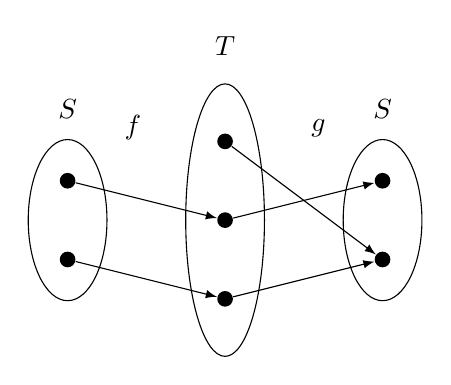
\begin{tikzpicture}
        \foreach \x in {1,2}
            \node[fill,circle,inner sep=2pt] (s\x) at (0,\x) {};
        \node[fit=(s1) (s2),ellipse,draw,minimum width=1cm,label={[anchor=north,above=22mm]270:$S$}, label={[anchor=north,above=22mm,right=6mm]270:$f$}] {};

        \foreach \x[count=\xi] in {0.5,1.5,...,3}
            \node[fill,circle,inner sep=2pt] (t\xi) at (2,\x) {};
        \node[fit=(t1) (t2) (t3),ellipse,draw,minimum width=1cm,label={[anchor=north,above=37mm]270:$T$}] {}; 

        \foreach \x[count=\xi] in {1,2}
            \node[fill,circle,inner sep=2pt] (s'\x) at (4,\x) {};
        \node[fit=(s'1) (s'2),ellipse,draw,minimum width=1cm,label={[anchor=north,above=22mm]270:$S$},label={[anchor=north,above=22mm,left=6mm]270:$g$}] {};
        
        \draw[-latex] (s1) -- (t1) ;
        \draw[-latex] (s2) -- (t2);
        \draw[-latex] (t1) -- (s'1);
        \draw[-latex] (t2) -- (s'2);
        \draw[-latex] (t3) -- (s'1);

    \end{tikzpicture}
\end{center}

\subsection*{d}
\begin{claim}
    $g$ is surjective.
\end{claim}

\begin{proof}
    $\forall s \in S, (g \circ f)(s) = id_S(s) = s$. We also have that $(g \circ f)(s) = g(f(s))$, so that $\forall s \in S, \exists t = f(s) \in T | g(t) = s$.
\end{proof}

\section*{Problem 6}

A function $f: A \rightarrow B$ can be expressed as its graph $\Gamma(f)$, which is the just the set $\{(a, f(a)) | a \in A\}$. 
Then, all functions $f: A \rightarrow B$ are sets containing elements of the form $(a, b) \in A \times B$. 
This implies that $\Gamma(f) \in \mathcal{P}(A \times B)$, which exists by the axiom of power sets. 

Note that we put $(a, b)$ as shorthand for a set $\{\{a\}, \{a,b\}\}$, and that products such as $A \times B$ are defined as all such $(a, b), a \in A, b \in B$. 

Then, by the axiom of specification, we pull out only the elements of $\mathcal{P}(A \times B)$ where it is a valid function graph. 
\begin{center}
    $\{\Gamma \in \mathcal{P}(A \times B) | (\forall a \in A, \exists (x,y) \in \Gamma \text{ s.t. } a = x)  \land (\neg\exists a \in A \text{ s.t. } (a, y), (a, y') \in \Gamma, y \neq y')\}$.
\end{center}

The set above is exactly $B^A$ if we equate functions and their graphs.

\section*{Problem 7}

There are $m^n$ elements in $B^A$, as each element of $A$ must be sent to an element in $B$, of which there are $m$. This is equivalent to making choosing $1$ from $m$ $n$ times, so that there are $m^n$ total choices for the function.

\section*{Problem 8}

\begin{proof}
    To show that $W$ is surjective, we can furnish a function $f: A \rightarrow B$ such that $W(f) = A'$ for any set $A' \in \mathcal{P}(A)$. 
    This function's graph is given exactly by 
    \begin{center}
        $\Gamma(f) = \{(a, 1) | a \in A'\} \cup \{(a, 0) | a \in A \setminus A'\}$.
    \end{center}
    
    In other words, for a function $f: A \rightarrow B$ such that 
    \[ f(a) = 
    \begin{cases} 
        1 & a \in A' \\
        0 & a \in A \setminus A' \\
   \end{cases} 
    \]

    To show that $W$ is injective, we will show that if $f, g \in B^A$ satisfy $W(f) = W(g) = A' \in \mathcal{P}(A)$ then $f = g$. 
    To show that $f = g$, we need to demonstrate that $\forall a \in A, f(a) = g(a)$. Since we have that $A' \cup A \setminus A' = A$ and $A' \cap A \setminus A' = \emptyset$, we have two cases for $a$.
    
    Firstly, if $a \in A'$, then $a \in f^{-1}(\{1\}) \implies f(a) = f(f^{-1}(1)) = 1$. Similarly, $a \in g^{-1}(\{1\}) \implies g(a) = 1$ such that $f(a) = g(a)$.
    
    Secondly, if $a \in A \setminus A'$, then $a \notin f^{-1}(\{1\}) \implies f(a) \neq f(f^{-1}(1)) \neq 1$. Similarly, $a \notin g^{-1}(\{1\}) \implies g(a) \neq 1$. However, both $f(a)$ and $g(a)$ are still members of $B$, meaning that they must be both equal to $0$.
    
    Thus, we have that $\forall a \in A, f(a) = g(a) \implies f = g$ and so $W$ is injective. $W$ is now shown to be both injective and surjective, so it must be bijective.
\end{proof}

\end{document}